\subsection{Combined Implementation}
An overall system block diagram of the final implementation of this project is shown in Figure \ref{finalBD}. This implementation may be broken down into several major components. At the top level, several blocks are used to connect the Zynq7 ARM Cortex A9 processing system to customized programmable logic using an AXI peripheral controller, as well as to peripherals such as the rangefinder and IMU using EMIO-GPIO and SPI-GPIO. 
\par
All programmable logic created for the rangefinder, IMU, and camera interface has been ported to a user-generated IP module named "custom logic", as shown in Figure \ref{finalBD}. This module connects directly to the stereo camera breakout board, and accepts rangefinder and IMU data from the programmable software via AXI interface. This customized IP core also accepts user inputs through the ZedBoard's switches, and supports outputs to the ZedBoard's LEDs and VGA interface. 
\par
\begin{figure}[!htb] 
	\centerline{
	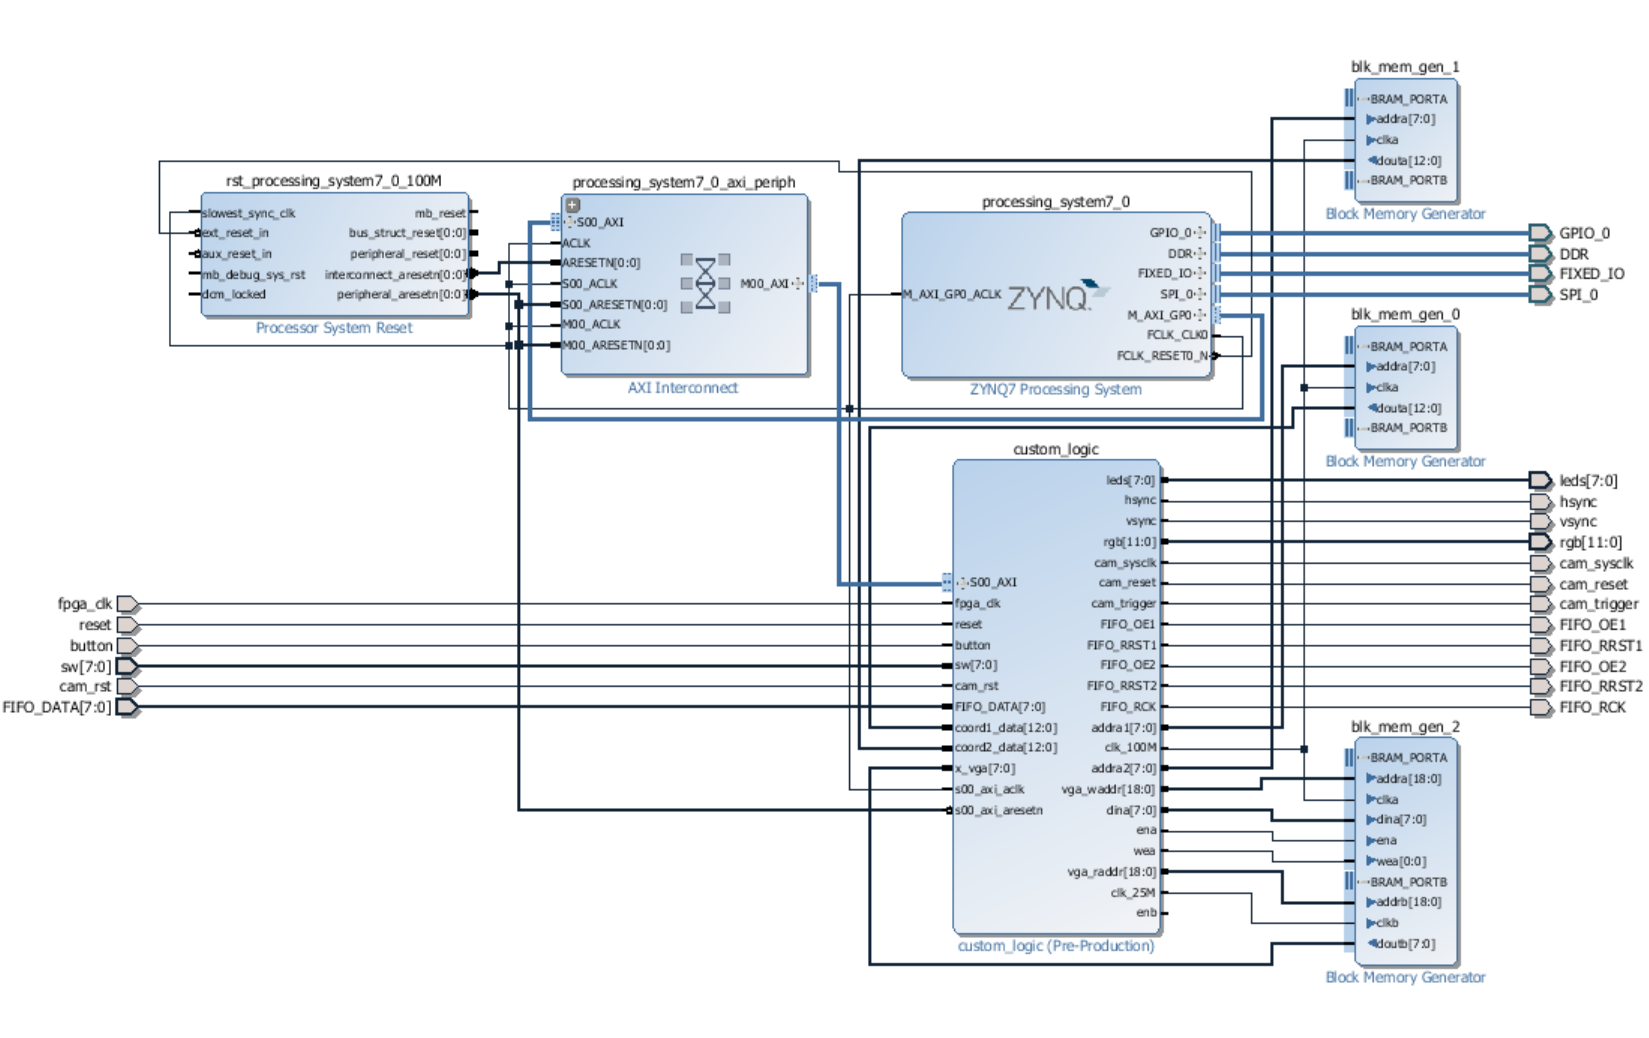
\includegraphics[width=1.25\linewidth, angle=90]{final_bd.png}
	}
	\caption{System Block Diagram}
	\label{finalBD}
\end{figure}
\par
The final hardware implementation of the project can be found in Figure 
\ref{finalHW}. This implementation supports several output modes based on the positions of the user switches, including a 3D disparity mode, camera image mode, rangefinder output mode, and combined 2D "floorplan" mode. Note that the VGA outputs of each mode are continuously updated in semi-realtime. 
\begin{figure}[H]  
 	\centerline{
	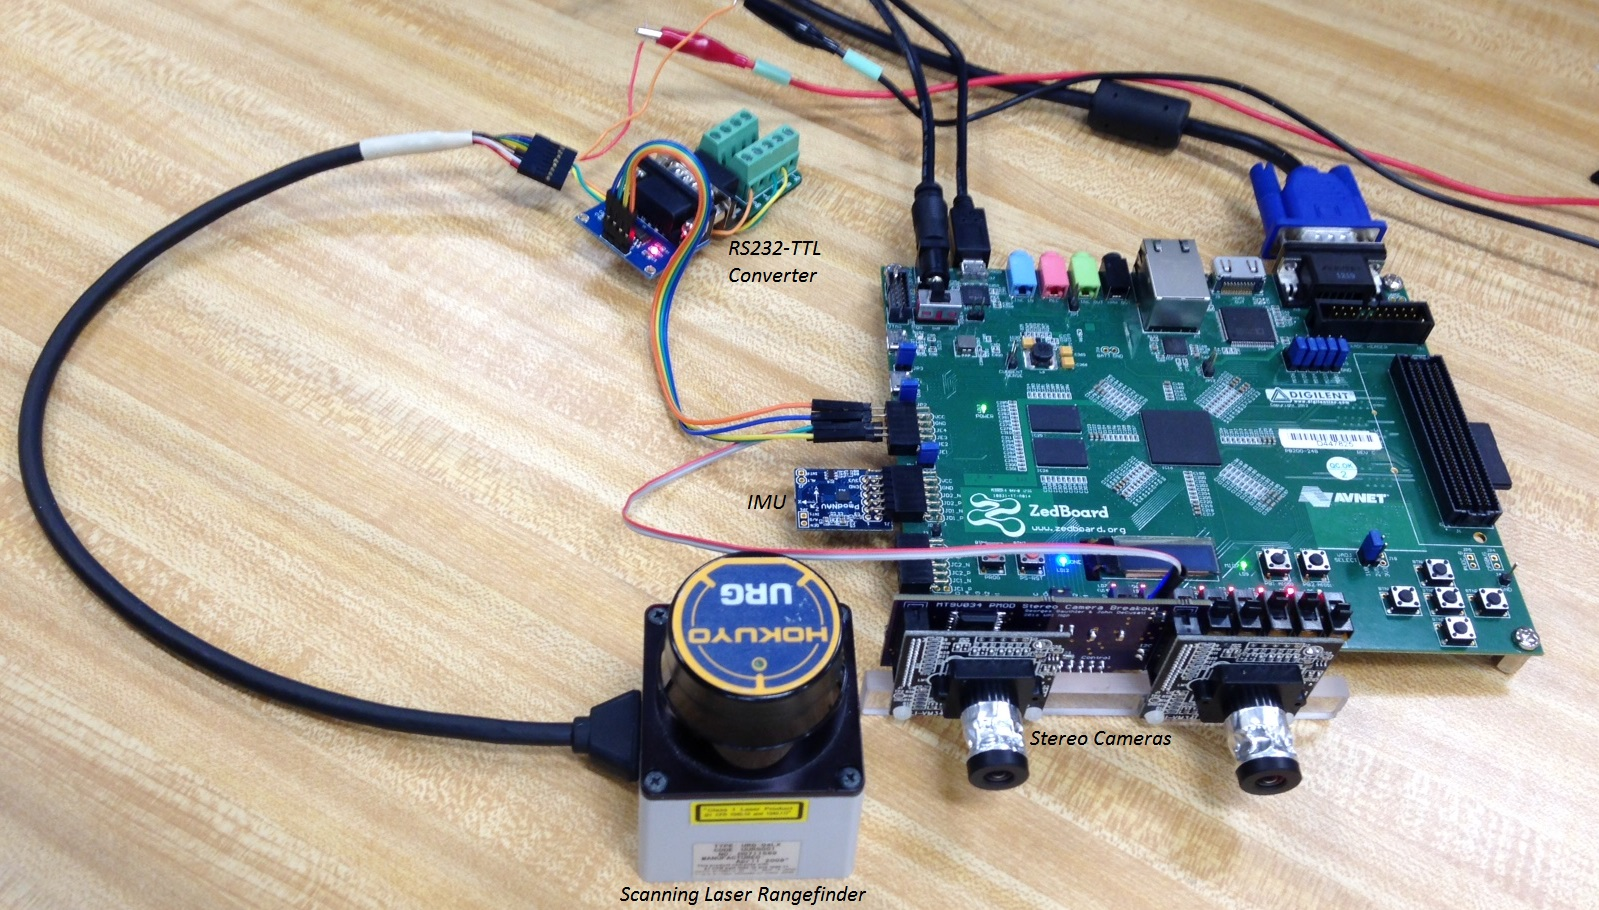
\includegraphics[width=0.85\linewidth]{setup.JPG}
	}
	\caption{System Hardware}
	\label{finalHW}
\end{figure}
\par
The 3D disparity output mode may be found in Figure \ref{disparityOutputs}a. In this mode, a windowed 384x288 pixel depth map is continuously updated to reflect the camera's current field of view. Figure \ref{disparityOutputs}b shows a modified version of this output consisting of depth information from a centrally-located horizontal line of pixels from this depth map that may then be correlated with data from the scanning laser rangefinder. 
\par
\begin{figure}[H] 
         \begin{subfigure}[h]{0.5\textwidth}
              \centerline{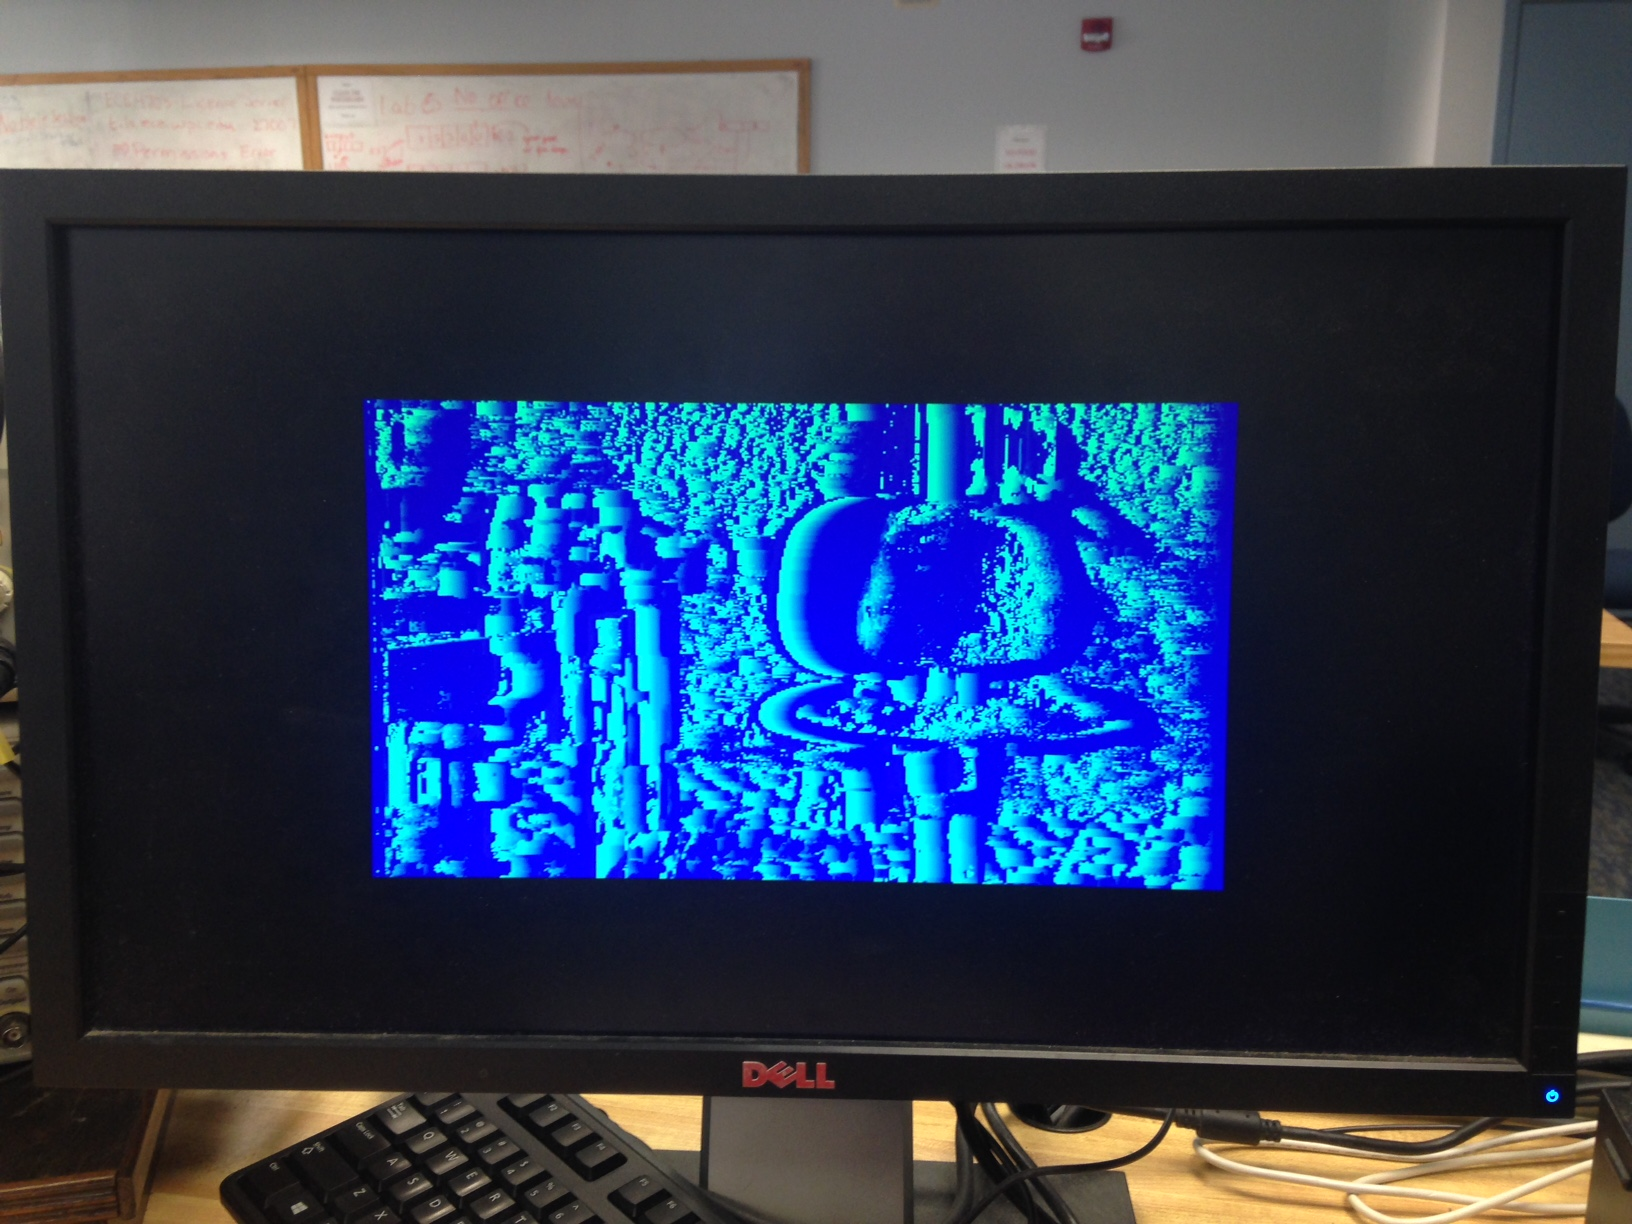
\includegraphics[width=1.0\textwidth]{disparity_mode.JPG}}
             \caption{Full Output}
         \end{subfigure}
         \begin{subfigure}[h]{0.5\textwidth}
             \centerline{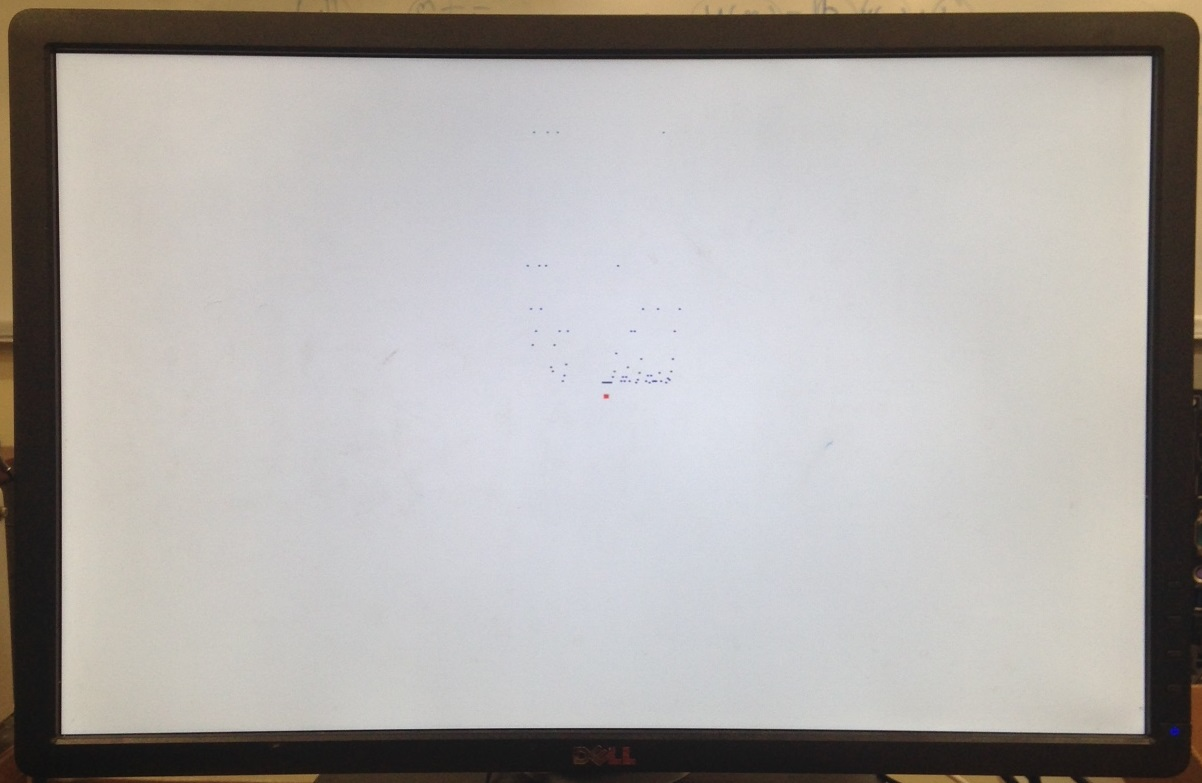
\includegraphics[width=1.0\textwidth]{disparity_line_mode.JPG}}
             \caption{Single Line Output}
         \end{subfigure}
\caption{Disparity Output Modes}
\label{disparityOutputs}
\end{figure}
\par
In order to aid in hardware debugging, an additional output mode has been included for showing the current camera images being used by the disparity algorithm, as shown in Figure \ref{camOutMode}. Note that the images captured are monochrome, and are being arbitrarily mapped to VGA colors due to a lack of grayscale color space.
\par
\begin{figure}[H]  
 	\centerline{
	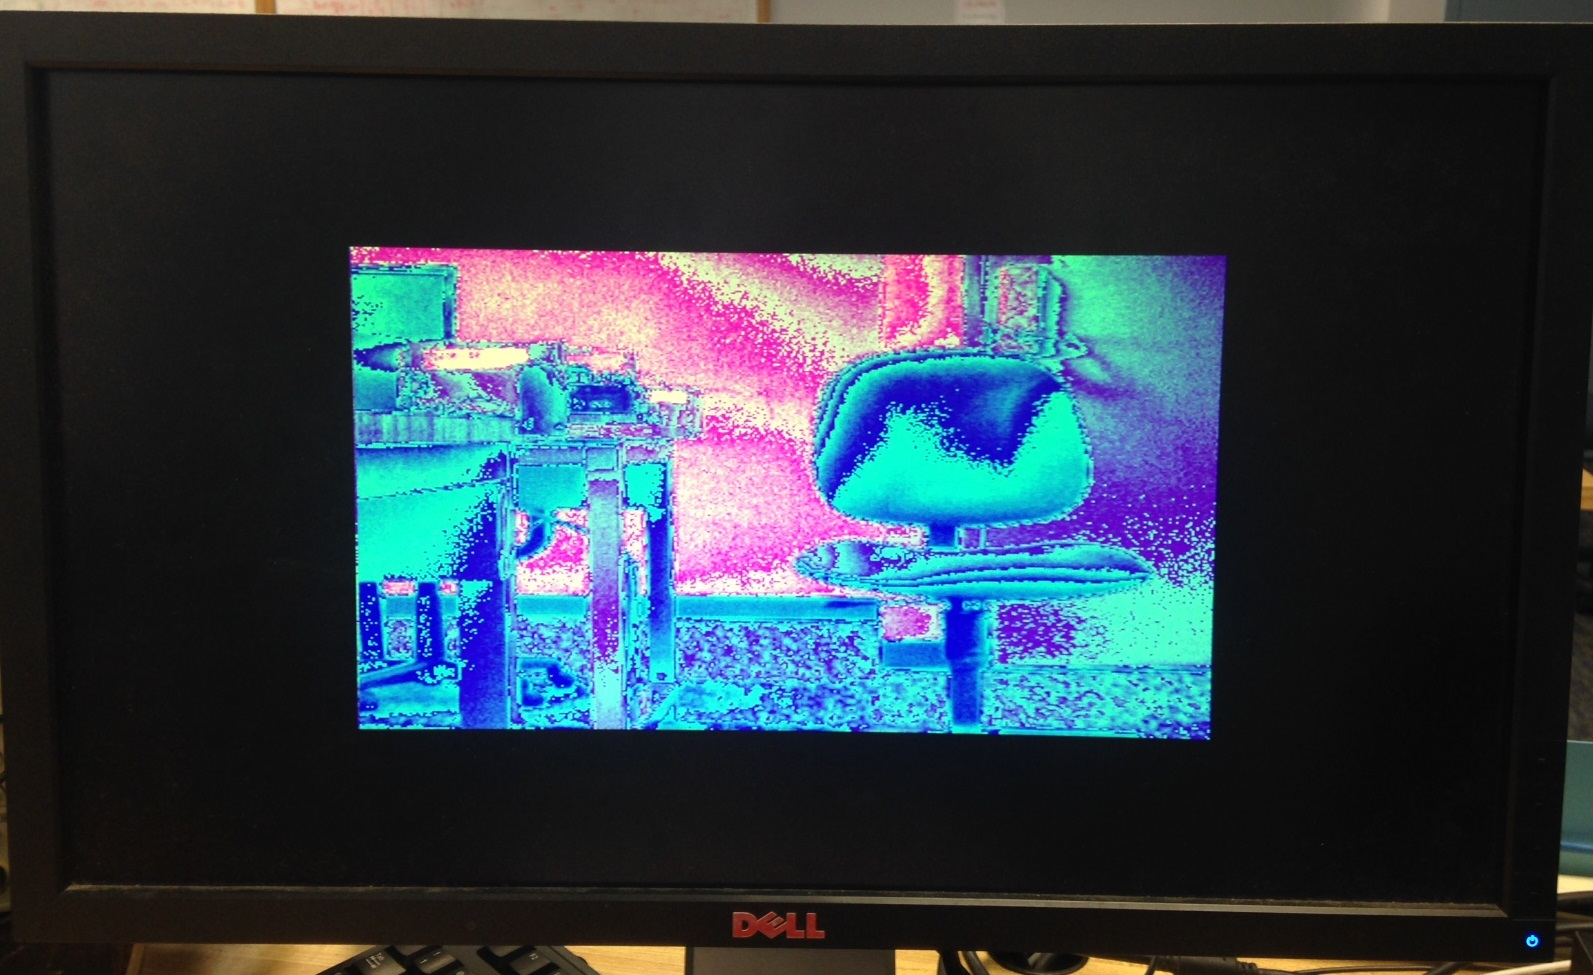
\includegraphics[width=0.5\linewidth]{camera_mode.JPG}
	}
	\caption{Raw Camera Data Mode}
	\label{camOutMode}
\end{figure} 
\par
The normal rangefinder output mode is shown in Figure \ref{rangeOutputs}a. In this mode, objects found by the scanning laser rangefinder are displayed in black. The entire scan is also referenced to the device's central location, shown in red. All rangefinder data is also pre-processed by the programmable software to include a compass offset from the IMU, with due north representing the center of the top of the VGA display.
\par 
A final output mode has also been included to incorporate disparity data with the 2D "floorplan" produced by the rangefinder. By combining data from both sensors, the stereo cameras are able to account for situations where the scanning laser rangefinder would be out of range due to its limitations on viewing distance. This output mode is shown in Figure \ref{rangeOutputs}b.

\begin{figure}[H] 
         \begin{subfigure}[h]{0.5\textwidth}
              \centerline{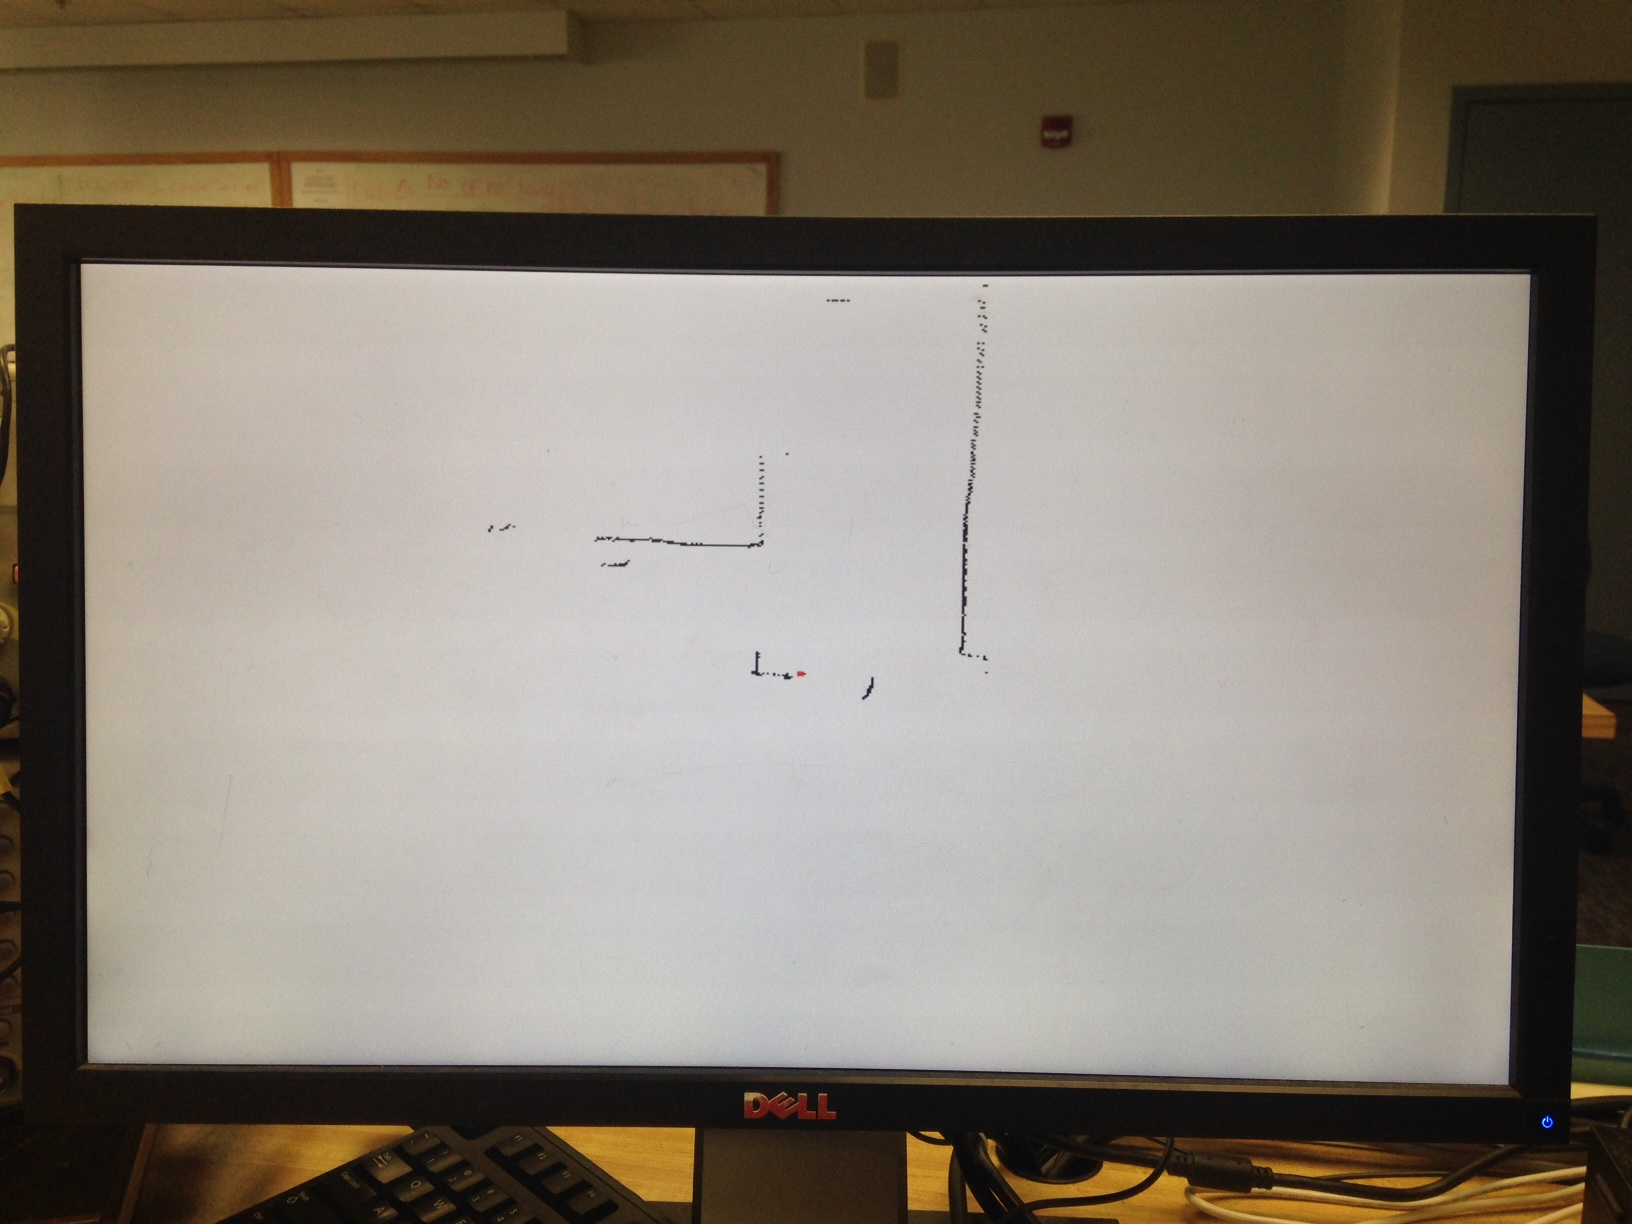
\includegraphics[width=1.0\textwidth]{rangefinder_mode.JPG}}
             \caption{Rangefinder Output}
         \end{subfigure}
         \begin{subfigure}[h]{0.5\textwidth}
             \centerline{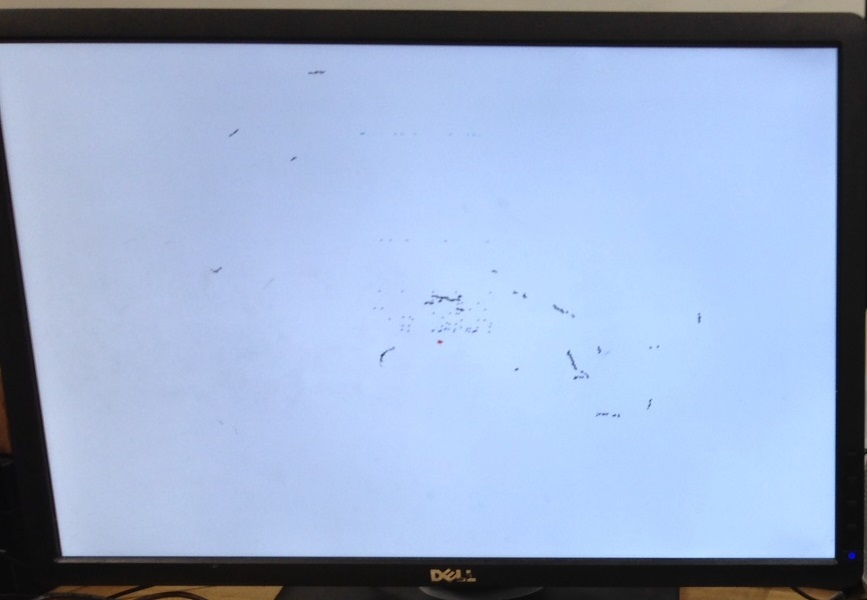
\includegraphics[width=1.0\textwidth]{combined_mode.JPG}}
             \caption{Combined Output}
         \end{subfigure}
\caption{2D "Floorplan" Output Modes}
\label{rangeOutputs}
\end{figure}
